
\documentclass[11pt]{article}

\marginparwidth 0.2in 
\oddsidemargin 0.1in 
\evensidemargin 0.1in 
\marginparsep 0.1in
\topmargin 0.1in 
\textwidth 6.5in \textheight 8 in

\usepackage{hyperref}  
\usepackage{listings}
\usepackage{array}
\usepackage{multirow}
\usepackage{attachfile}
\usepackage{lscape}
\usepackage{graphicx}
\usepackage{etoolbox}
\usepackage[usenames,dvipsnames]{xcolor}
\usepackage{transparent}

\makeatletter
\patchcmd{\@maketitle}{\vskip 2em}{\vspace*{-3cm}}{}{}
\makeatother

\author{İbrahim Burak Tanrıkulu, 21827852}
\title{BBM434 Gömülü Sistemler Lab.\\Deney 2}

\lstset {language=C, tabsize=4, backgroundcolor =  \transparent{.3}\color{gray}}
\newcommand\tab[1][1cm]{\hspace*{#1}}

\begin{document}
\maketitle

\section{Çalışma ortamını hazırlama}
Gömülü sistemlere giriş yapmak için öncelikle çalışma ortamımızı hazırlamamız gerekiyor. Ben çalışma ortamımda birden fazla program kullanacağım. 
\begin{itemize}
\item {\bf Arduino IDE}\\
Arduino IDE ile Arduino kartları için yazılım yazıp bu kartlara yükleyebiliyoruz. Ayrıca bu IDE'nin bize sunduğu örnek kodlar da var.\\
\begin{minipage}{0.4\textwidth}

\includegraphics[width=3cm]{arduino_ide.png}
\centering
\end{minipage}
\begin{minipage}{0.4\textwidth}
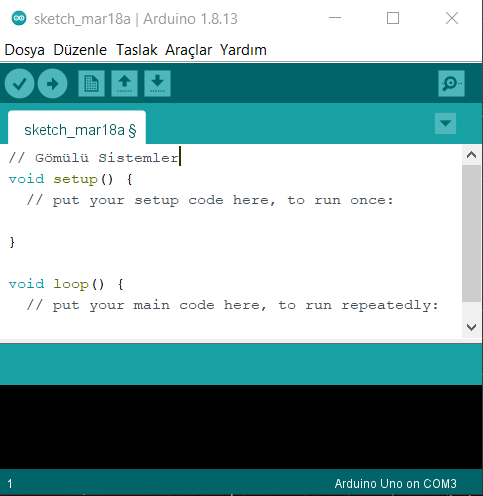
\includegraphics[width=8cm]{arduino.png}
\centering
\end{minipage}
\item {\bf Proteus}\\
Proteus ile yapmayı düşündüğümüz sistemin şemasını çizebilir, gerekirse kod yazabilir ve sisteminizi simüle edebilirsiniz. Ayrıca PCB tasarımını yapıp 3 boyutlu olarak görüntileyebilirsiniz.\\
\begin{minipage}{0.45\textwidth}
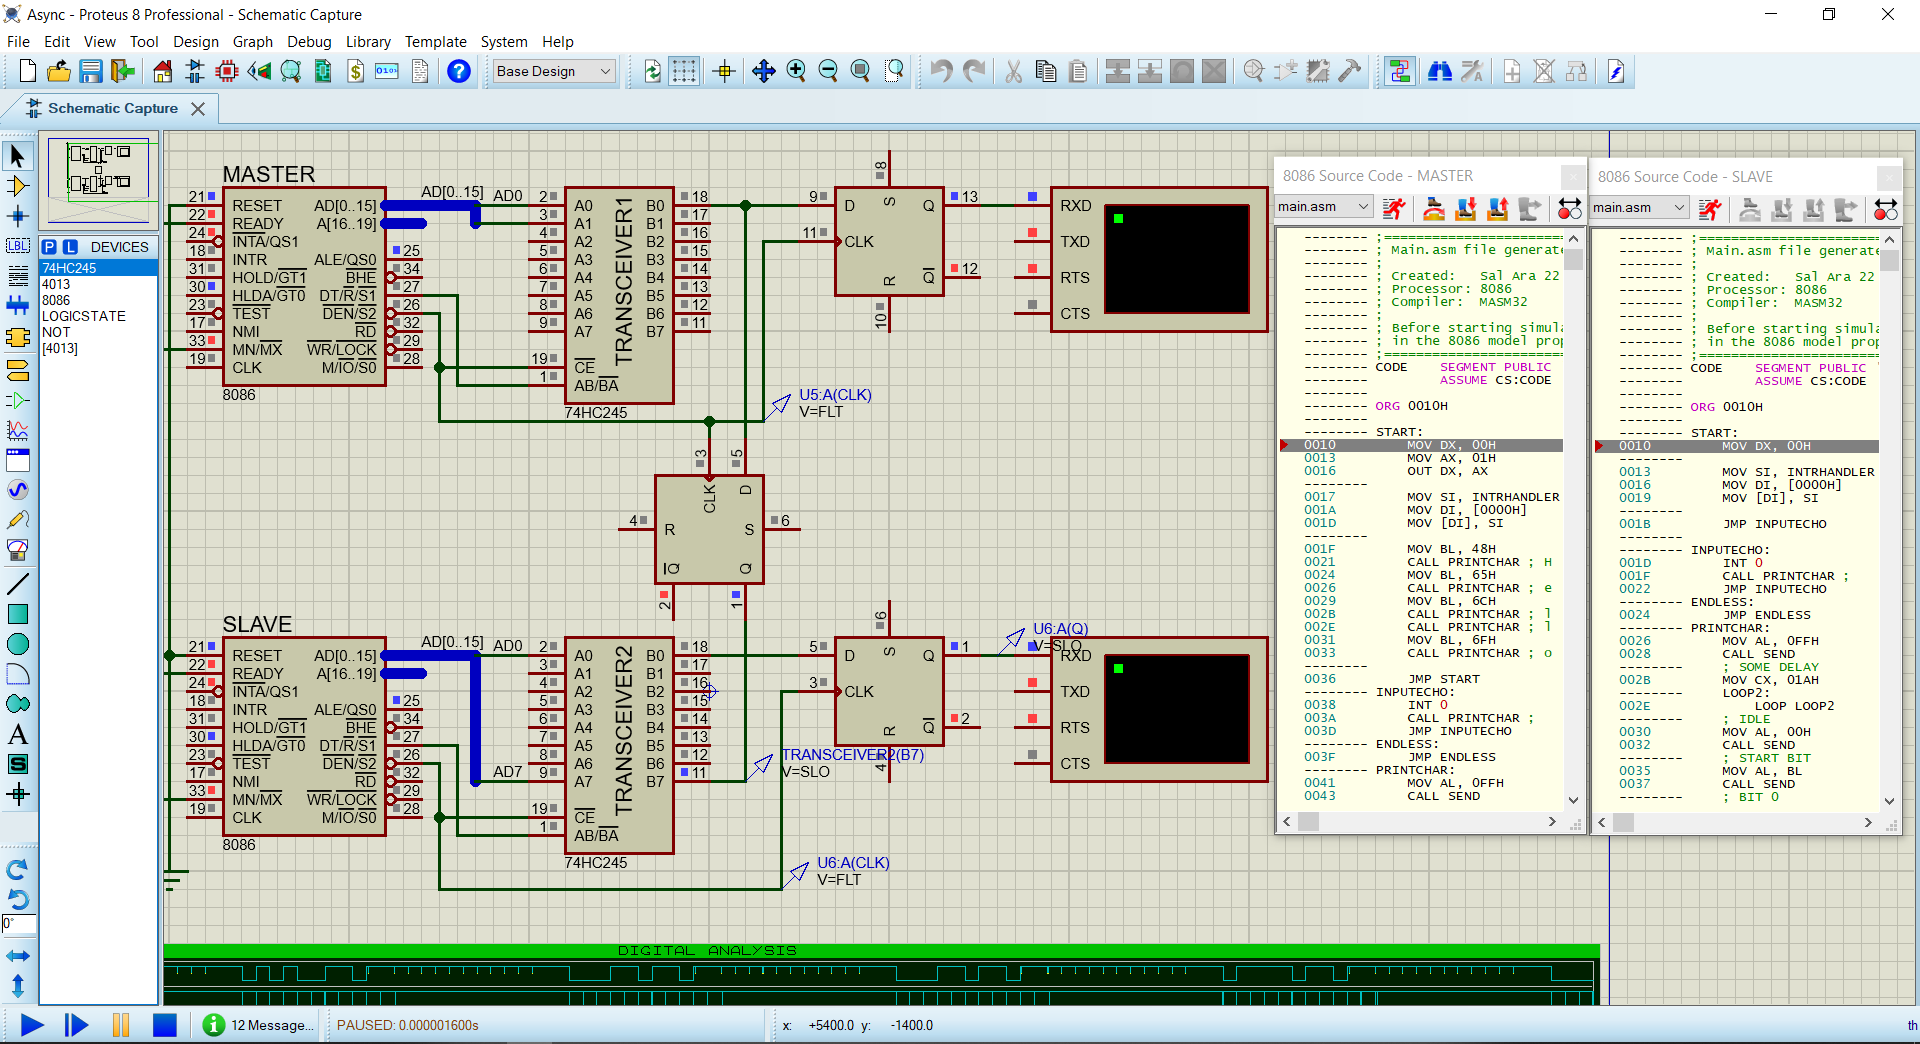
\includegraphics[width=7cm]{proteus.png}
\centering
\end{minipage}
\begin{minipage}{0.5\textwidth}
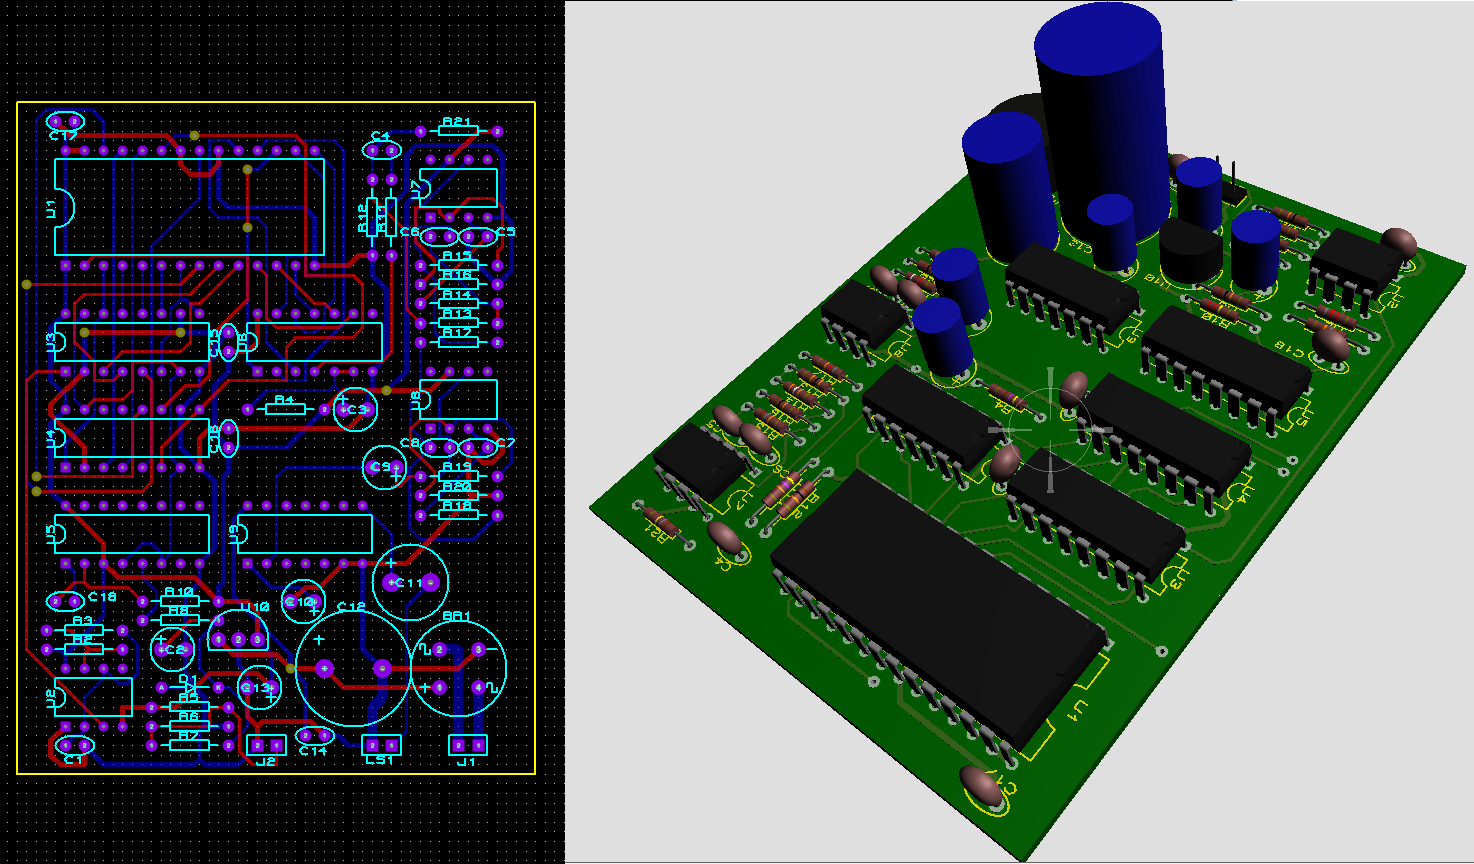
\includegraphics[width=7cm]{proteus2.png}
\centering
\end{minipage}
\item {\bf Fritzing / Tinkercad}\\
Bu iki program birbirlerine çok benziyor. Fritzing'i indirip bilgisayarınıza kurarken; Tinkercad bir internet sitesidir, online kullanırsınız. Temel olarak Arduino projelerinizi çizip, kodunuzu yazıp bu ortamı simule etmeye yararlar. Görünüşleri de birbirine çok benzer. 
\begin{minipage}{0.45\textwidth}
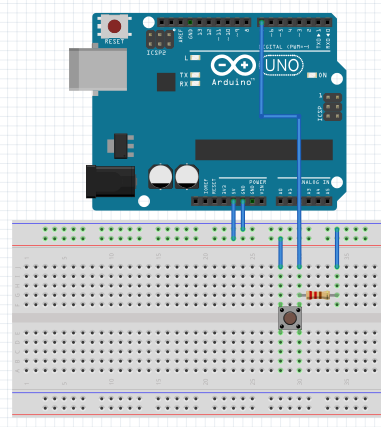
\includegraphics[width=7cm]{fritzing.png}
\centering
\end{minipage}
\begin{minipage}{0.5\textwidth}
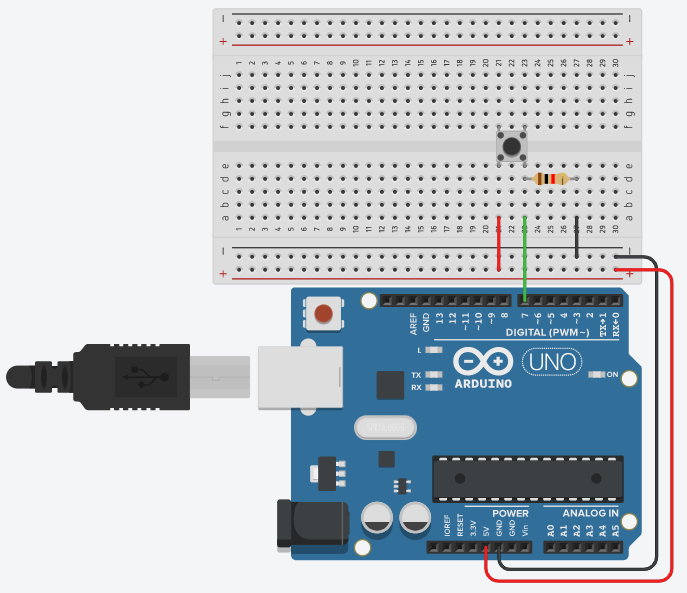
\includegraphics[width=7cm]{tinkercad.png}
\centering
\end{minipage}
\item {\bf Matlab}\\
Mühendisler birçok projede matematiksel işlemlere ihtiyaç duyar. Matlab (adından da anlaşılacağı gibi) matematik konusunda çok iyi bir programdır. Programlama dilleri ile matematiksel işlemler arasınaki iletişimi sağlar.\\~\\
\begin{minipage}{0.5\textwidth}

\includegraphics[width=7cm]{matlab.jpg}
\centering
\end{minipage}
\end{itemize}
\end{document}
